\documentclass[sans serif,9pt,xcolor=dvipsnames]{beamer}%tipo de documento

\usetheme{Copenhagen}% tema a utilizar
%\useoutertheme{infolines}
%\usecolortheme[RGB={50,93,16}]{structure}
\usecolortheme[RGB={123,16,64}]{structure}
\useinnertheme{rectangles}
%79 168 51
\setbeamercovered{transparent}
%para el difumidado de las transparencias
\beamertemplateshadingbackground{gray!20}{purple!20}
% papaquetes personales
\usepackage[spanish]{babel}%paquete de idioma
%la utilizacion de la instruccion anterior puede llevar a que existan errores en los demás paquetes para ello:
\renewcommand{\contentsname}{Contenido}
\renewcommand{\partname}{Parte}
\renewcommand{\appendixname}{Apéndice}
\renewcommand{\figurename}{Figura}
\renewcommand{\tablename}{Tabla}
\renewcommand{\abstractname}{Resumen}

\usepackage[utf8]{inputenc}% utf8 permite la utilizacion de tildes y Ñ directamente del teclado si la distribucion es utf8. Pero si se tiene otra distribucion, el argumento será latin1
\usepackage{geometry} % para margenes
\usepackage{graphicx} % para colocacion de figuras
\usepackage{color}% para colorear el texto
\usepackage{hyperref}%para hacer referencias a las direcciones de paginas en internet
\usepackage{url}% para escribir una URL
\usepackage{ragged2e}

\usepackage{listings}

\begin{document}
\title[UIDE - IEEE - RNR2015]{\textbf{\Huge Programación Literaria Investigación Reproducible y Software Libre}}  
\author[Ing. Milton Labanda, Mg.]{Ing. Milton Labanda, Mg.}
\institute[UIDE Informática]{Carrera de Ingeniería Informática y Multimedia\\ Universidad Internacional del Ecuador}

\setbeamerfont{title}{shape=\itshape,family=\rmfamily}%cambiar tipo de letra
%\setbeamercolor{title}{fg=blue!80!black,bg=green!20!white}%comabiar color de letra y color de cuadro

%marco para el pie en el titulo
\begin{frame}
\hfill {Reunión Nacional de Ramas IEEE RNR2015}
\titlepage
\begin{center}
%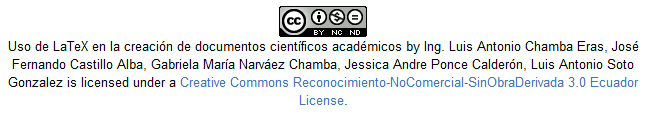
\includegraphics[height=0.2\textheight]{imagenes/licencia.PNG} 
\end{center}

\end{frame}

%marco para el contenido
\AtBeginSection [<+-| alert@+>]{
\begin{frame}{Outline} %<beamer>
\frametitle {Contenido}
\tableofcontents [currentsection]
\end{frame}}


\section{Programación Literaria}
\subsection{Historia}
\begin{frame}
\frametitle{Historia}
\begin{block}{Como empieza todo?}
\begin{columns}
\column{.1\textwidth} \hspace{0.7cm}
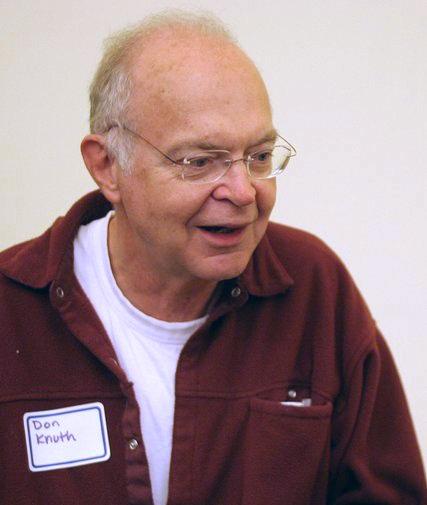
\includegraphics[width=1.8cm]{imagenes/donald.jpg}
\column{.8\textwidth}
\justifying
"Computer programs should be written in a combination of the programming language (the usual source code) and the natural language, which explains the logic of the program". \textbf{\textit{Donald Knuth}}
\end{columns}
\end{block}

\begin{block}{El objetivo}
\begin{columns}
\column{.1\textwidth} \hspace{0.7cm}

\includegraphics[height=1.5cm]{imagenes/book.png} 
\column{.8\textwidth}
\justifying
I believe that the time is ripe for significantly better documentation of programs, and that we can best achieve this by considering programs to be works of literature. Hence, my title: "Literate Programming" \textbf{\textit{Donald Knuth}}
\end{columns}
\end{block}

\end{frame}

\begin{frame}
\frametitle{Historia}

\begin{block}{WEB}
\begin{columns}
%\column{.1\textwidth} %\hspace{0.7cm}
% % %
\includegraphics[width=1.8cm]{imagenes/latex.png} 
\column{.8\textwidth}
\justifying
Primera herramienta de implementación de lo que se conoció como Programación Literaria. Producía código PACAL compilable y la documentación formateada usando Tex
\end{columns}
\end{block}

\begin{block}{CWEB}
\begin{columns}
%\column{.1\textwidth} %\hspace{0.7cm}
% % %
\includegraphics[width=1.8cm]{imagenes/latex.png} 
\column{.8\textwidth}
\justifying
Descendiente del entorno WEB usa en cambio C como lenguaje de programación pero el mismo Tex para la generación de la documentación
\end{columns}
\end{block}
\end{frame}

\subsection{?`Qué es la Programación Literaria o Estadística?}
\begin{frame}
  \frametitle{?`Qué es la Programación Literaria ?}
\begin{itemize}
\justifying
\item Paradigma cotrario a la programación tradicional: En vez de escribir código que contiene documentación el programador literario escribe documentación que contiene código. 
\bigskip
\item Los Programas literarios pueden ser tejidos (WEAVED) para producir documentos legibles para los humanos y enredados (TANGLED) para producir documentos legibles para las máquinas"

\end{itemize}
\end{frame}

\subsection{Elementos de la Programación Literaria}
\begin{frame}
  \frametitle{Elementos de la Programación Literaria}
\begin{itemize}
\justifying
\item Cada "trozo" de código fuente carga datos y calcula resultados mientras que el código de presentación formatea la salida
\bigskip
 \item Consecuentemente el paradigma de la programación literaria requiere: 
\begin{enumerate}
\item Un lenguaje de documentación (human readable)
\item Un lenguaje de programación (machine readable)
\end{enumerate}
\end{itemize}
\end{frame}

\subsection{Ejemplos de implementaciones o entornos}
\begin{frame}
  \frametitle{Ejemplos de implementaciones o entornos}
\begin{itemize}
\justifying
\item Sweave = \LaTeX + R
\bigskip
\item  knitr = HTML + R
\bigskip
\item  Jupyter = HTML + Python
\bigskip
\item  Rambutan = \TeX + Java
\bigskip
\item  CoffeScript (Markdown + CoffeScript)
\end{itemize}
\end{frame}

\begin{frame}
\frametitle{Ejemplo knitr}
%\begin{block}{}
\begin{columns}
\column{.4\textwidth} \hspace{1cm}
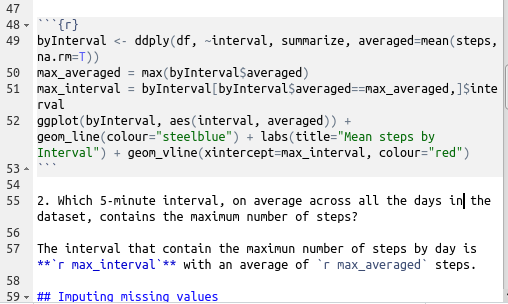
\includegraphics[scale=0.3]{imagenes/rmd_input.png}
\column{.4\textwidth}
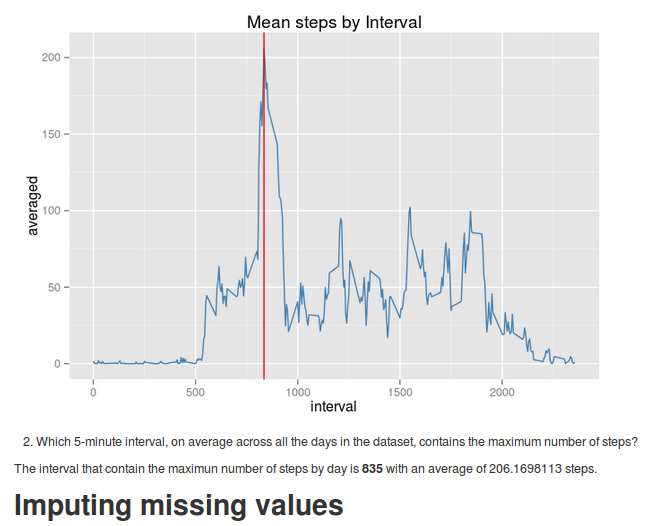
\includegraphics[scale=0.24]{imagenes/rmd_output.png} 
\end{columns}
%\end{block}
\end{frame}

\begin{frame}
\frametitle{Ejemplo Jupyter (IPython Notebook)}
%\begin{block}{}
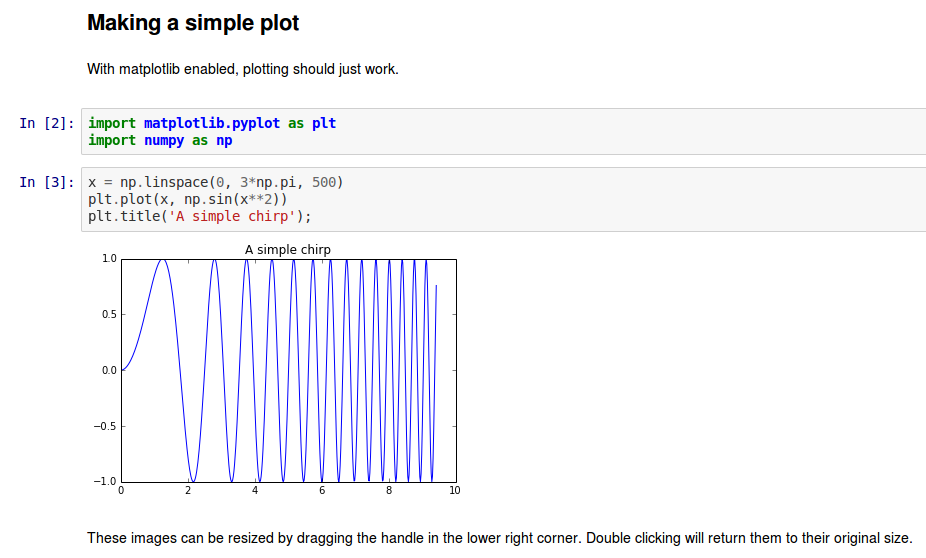
\includegraphics[scale=0.3]{imagenes/pynb.png} 
%\end{block}
\end{frame}


\section{Investigación Reproducible}
\subsection{La Investigación y el Análisis de Datos}
\begin{frame}
\begin{block}{Según Sampieri}
\Large El \textbf{Análisis de Datos} es el 9no paso dentro de la \textbf{Investigación}
\end{block}
\end{frame}


\begin{frame}
\frametitle{Estructura de un Análisis de Datos}
\justifying
\begin{block}{}
\begin{itemize}
\item Definir la pregunta
\item Definir el dataset ideal
\item Determinar que datos se pueden acceder
\item Obtener los datos
\item Limpiar los datos
\item Análisis de Datos exploratorio
\item Modelamiento/predicción estadístico
\item Interpretar los resultados
%\item Mejorar los resultados
\item Escribir/sintetizar los resultados
\item Crear código reproducible
\end{itemize}
\end{block}
\end{frame}

\begin{frame}
\frametitle{Encadenamiento de la investigación}
\justifying
%\begin{block}
\begin{center}
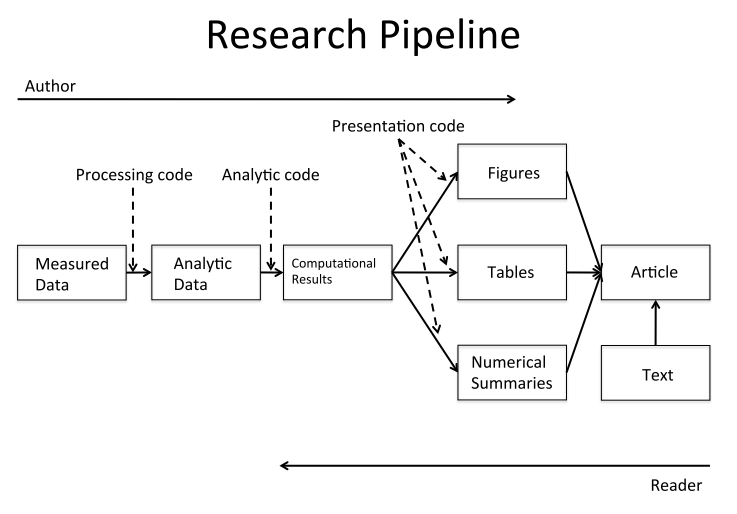
\includegraphics[scale=0.35]{imagenes/research_flow.png}
\end{center}
%\end{block}
\end{frame}

\begin{frame}
\frametitle{Los actores del Análisis de Datos}
\justifying
\begin{block}{Autores} 
\begin{itemize}
  \item Desean hacer su investigación reproducible
  \item Quieren herramientas de IR que hagan su vida más facil ("no muy dura")
  \item Relizan considerables esfuerzos para publicar su datos. E: servidor web
  \item Entonces => Con IR colocan solo lo mínimo en la Web así como materiales suplementarios en las revistas o en bases de datos centrales
\end{itemize}
\end{block}
\begin{block}{Lectores} 
\begin{itemize}
  \item Quieren reproducir y posiblemente expandir los descubrimientos de interés
  \item Quieren herramientas de IR para hacer su vida más fácil ("no muy dura")
  \item Deben descargar datos y juntar las piezas: que datos va con qué codigo?
  %\item Pueden no tener los mismos recursos que los autores
  \item Entonces => Descargan los datos y analizan, juntan el software y ejecutan
\end{itemize}
\end{block}
\end{frame}

\subsection{La Investigación necesita ser reproducible}
\begin{frame}
\frametitle{?`Por qué necesita ser Reproducible?}
\begin{block}{... hoy más que nunca}
\begin{itemize}
\justifying
\item Las nuevas tecnologías incrementan las colecciones de datos cada vez más
\item Los datos son más complejos y extremadamente multidimensionales
\item Las bases de datos existentes pueden ser mezcladas dentro de "mega bases de datos"
\item La capacidad de cómputo es altamente incrementable permitiendo análisis mas sofisticados
\item Para cada campo 'X' existe un campo "Computacional 'X'
\end{itemize}
\end{block}
\end{frame}

\begin{frame}
\frametitle {?`Para qué debe ser Reproducible?}
\justifying
\begin{block}{Debe}
\LARGE Hacer los \textbf{datos analíticos} y el \textbf{código computacional} disponibles para que otros puedan reproducir los descubrimientos
\end{block}
\end{frame}

\subsection{Análisis de Datos y Programación Literaria}
\begin{frame}
\frametitle{Elementos de un Análisis de Datos moderno }
\justifying
\begin{block}{}
\begin{itemize}
\item Datos
  \begin{itemize}
  \item Datos crudos (raw)
  \item Datos procesados
  \end{itemize}
\item Figuras
\begin{itemize}
  \item Figuras exploratorias
  \item Figuras finales
\end{itemize}
\item Código
\begin{itemize}
  \item Scripts borrador/no usados
  \item Scripts finales (R, Julia, Python ...)
  \item Scripts Literarios 
\begin{itemize}
    \item Archivos .rmd (R markdown)
    \item Archivos .ipynb (Jupyter/IPython notebooks)
\end{itemize}    
\end{itemize}
\item Texto:
\begin{itemize}
  \item Archivo de ayuda (README)
  \item Texto del análisis/reporte (pdf, html) generado comunmente por  herramientas de programación literaria
 \end{itemize}
\end{itemize}
\end{block}
\end{frame}

\begin{frame}
\frametitle{Estructura mínima de un reporte de Análisis de Datos}
\justifying
\begin{block}{}
\begin{itemize}
\item \Large Titulo
\item \Large Introducción/motivación
\item \Large Metodos (estadísticos)
\item \Large Resultados
\item \Large Conclusiones
\end{itemize}
\end{block}
\end{frame}


\section{Software Libre}
\begin{frame}
\frametitle {Entronos y herramientas modernas}
\justifying
\begin{block}{Jupyter(IPython Notebook)}
\begin{columns}
\column{.1\textwidth} \hspace{0.7cm}

\includegraphics[width=2.2cm]{imagenes/jupyter.png} 
\column{.8\textwidth}
\begin{itemize}
\justifying
\item Creado por Fernando Perez (estudiante de ingeniería aeronáutica)
\item Entorno completo de computación interactiva en el browser
\item HTML o Markdown + Python o Julia
\item Permite binding hacia otros lenguajes como: R, ruby, shell, ...
\item Exporta los documentos resultantes hacia: PDF, HTML, Latex o reveal.js 
\item \textbf{nbviewer} [\url{http://nbviewer.ipython.org/}] el servicio de publicación gratuito de notebooks en la Web 
\end{itemize}
\end{columns}
\end{block}
\end{frame}

\begin{frame}
\frametitle {Entornos y herramientas modernas}
\justifying
\begin{block}{knitr + RStudio}
\begin{columns}
\column{.1\textwidth} \hspace{0.7cm}

\includegraphics[width=2.3cm]{imagenes/knitr.png} 
\column{.8\textwidth}
\begin{itemize}
\justifying
\item \textbf{knitr} desarrollado por Yihui Xie al realizar su trabajo de graduación
\item Es una librería escrita en R y para R
\item HTML(o \LaTeX o Markdown) + R 
\item Orientado a mitigar las limitaciones de SWEAVE.
\item Puede exportar a PDF, HTML o Word
\item \textbf{knitr} es integrable con el IDE \textbf{RStudio}
\item \textbf{Rpubs} [\url{http://rpubs.com}] su servicio de publicación gratuito de RStudio en la Web
\end{itemize}
\end{columns}
\end{block}
\end{frame}

\begin{frame}
\frametitle {Entornos y herramientas modernas}
\justifying
\begin{block}{git}
\begin{columns}
\column{.1\textwidth} \hspace{0.7cm}

\includegraphics[width=2.3cm]{imagenes/git.png} 
\column{.8\textwidth}
\begin{itemize}
\justifying
\item \textbf Desarrollado por Linus Torvalds en el 2005 
\item Herramienta de control de versiones distribuida
\item Rápido y pequeño
\item Abundantes comandos que permiten el trabajo colaborativo 
\item Cuarda el rastro de los cambios muy detalladamente
\item Git LFS: extensión para manegar archivos de gran tamaño 
\end{itemize}
\end{columns}
\end{block}
\end{frame}

\begin{frame}
\frametitle {Entornos y herramientas modernas}
\justifying
\begin{block}{github}
\begin{columns}
\column{.1\textwidth} \hspace{0.7cm}

\includegraphics[width=2.3cm]{imagenes/github.png} 
\column{.8\textwidth}
\begin{itemize}
\justifying
\item Originalmente conocida como Logical Awsome
\item Plataforma de desarrollo de software colaborativo, pero, con millares de repositorios que contienen codigo y datos de experimentos reproducibles
\item El código se alamacena de forma pública con la posibilidad de hacerlo privado
\item Utilizado en academia e investigación: escuela tradicional, MOOCS, ciencias,..
\item Github alcanzó \textbf{1 millón} de repositorios en el \textbf{2010}, \textbf{2 millones} en el \textbf{2011}, \textbf{10 millones} en el \textbf{2013} y llegando a \textbf{21 millones} de repositorios en Abril del \textbf{2015} y \textbf{9 millones de usuarios}
\end{itemize}
\end{columns}
\end{block}
\end{frame}

\section{Demos}
\begin{frame}
\frametitle {}
\centering \Huge Demos
\end{frame}

%++++++++++++++++++++++++++

%\section{Enlaces de Ayuda}
%\begin{frame}
%\frametitle {Enlaces de Ayuda}
%\begin{thebibliography}{10}
%\bibitem{  } Alex Borbón A., Walter Mora F.
%\newblock{ \LaTeX Composición, Diseño Editorial, Gráficos,
%Inkscape, Tikz y Presentaciones Beame} 2012
%\newblock 
%\url{http://www.tec-digital.itcr.ac.cr/revistamatematica/Libros/LATEX/LaTeX_2011.pdf}
%\end{thebibliography}
%\end{frame}

\begin{frame}
\frametitle {Créditos}
\begin{center}
\textbf{\textit{Expositor}}\\
Ing. Milton Leonardo Labanda Jaramillo, Mg.\\
\vspace{0.25 cm}
\textbf{@miltonlab}\\
\vspace{0.15 cm}

\includegraphics[scale=0.25]{imagenes/twitter47.png} \hspace{0.5 cm}

\includegraphics[scale=0.25]{imagenes/linkedin12.png} \hspace{0.5 cm} 
\includegraphics[scale=0.25]{imagenes/github17.png}\\
\vspace{1 cm}

\includegraphics{imagenes/uide.png} \\
\textbf{Universidad Internacional del Ecuador sede Loja\\
Escuela de Informática y Multimedia\\
2015
}
	\end{center}
\end{frame}

\end{document}
\textbf{}